\documentclass[a4paper,11pt]{article} 

% ===== Algunos paquetes a ser usados =====

% para poder escribir con tildes   
\usepackage[T1]{fontenc}           
\usepackage[utf8]{inputenc}        
\usepackage[spanish]{babel}        

\spanishdecimal{.}        
\usepackage{times}        

\usepackage{animate}        

% fuentes para escribir símbolos 
\usepackage{amsfonts}            
\usepackage{amssymb}             
\usepackage{amsthm}              
\usepackage{mathrsfs}            
\usepackage[centertags]{amsmath}    

% inclusión de graficos    
\usepackage{graphicx}      

% símbolo de grados    
\newcommand{\grad}{\hspace{-2.5mm}$\,\phantom{a}^{\circ}\,$}        

% ==================================== 

% ========= Referencias ==========           
\usepackage{hyperref}                        
% ================================           

% ========= Color ==========           
\usepackage[usenames,dvipsnames]{color}                         
% ================================           

% ===== Ajuste layout pagina =====           
\textheight=23cm                            
\textwidth=18cm                              
\topmargin=-1cm                              
\oddsidemargin=-1cm                           
\parindent=0mm                               
\usepackage{fancyhdr}                        
% ================================           

% ========= Comandos ==========           
\newcommand{\ds}{\displaystyle}         
\def\x{{\bf x}}                         
% ================================           

% ========= Tablas y otros ==========           
%\usepackage[table]{xcolor} % Sirve para poner letras con colores y colorear tablas            
\addto\captionsspanish{ \renewcommand{\tablename}{Tabla}} %Uso tabla en vez de cuadro        
\addto\captionsspanish{ \renewcommand{\appendixname}{Apéndice}}                               
%\addto\captionsspanish{ \renewcommand{\appendixpagename}{Apéndice}}                         
%\addto\captionsspanish{ \renewcommand{\appendixtocname}{Apéndice}}                          
%\addto\captionsspanish{ \renewcommand{\lstlistingname}{Rutina}}                             
\usepackage{array}                                                                               
\newcolumntype{C}[1]{>{\centering\let\newline\\\arraybackslash\hspace{0pt}}m{#1}}         
\newcolumntype{L}[1]{>{\raggedright\let\newline\\\arraybackslash\hspace{0pt}}m{#1}}       
\newcolumntype{R}[1]{>{\raggedleft\let\newline\\\arraybackslash\hspace{0pt}}m{#1}}        
\usepackage{booktabs}                                                                            
\usepackage{longtable}                                                                            
% ================================           

\newpage  

\begin{document}      

% == Encabezado y pie de pagina ==           
\pagestyle{fancy}                            
\cfoot{}                                     
\lhead{Nombre del proyecto}                  
\lfoot{\footnotesize Reacción Lineal}      
\rfoot{Pág. \thepage}                        
% ================================           

% ======== Texto ==========  

\begin{minipage}[t]{1\textwidth}      
\vspace{0.5mm}      
\noindent      
Curso de Elasticidad 2014 \\     
Ingeniería Civil - Plan 97 \\      
Materia: Resistencia de Materiales      

\begin{center}      
\textbf{\Large{ Archivo de entrada:}}\Large{ \verb+torre.txt+}  \\      
\large{Nombre del proyecto\\}       
\today\\      
IETFEM v2.11      
\vspace{-2.9cm}      
\end{center}      
\end{minipage}      
\hspace{-2cm}      
\begin{minipage}[t]{.1\textwidth}      
\vspace{0.0mm}      

\includegraphics[width=.95\textwidth]{../../../../../../sources/Figs/logo_udelar}      
\end{minipage}      

\vspace{1cm}       

\hspace{1.5cm}       
\begin{center}       
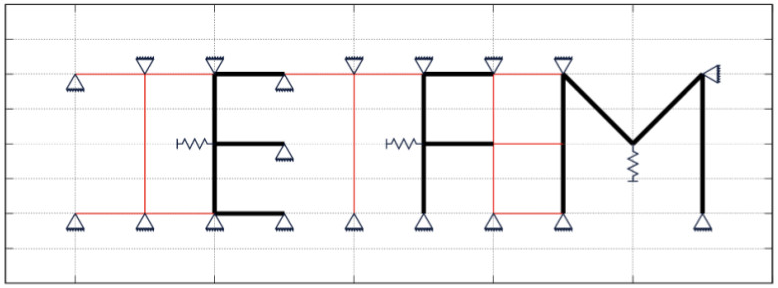
\includegraphics[width=.95\textwidth]{../../../../../../sources/Figs/logo_ietfem}      
\end{center}       
\vspace{0.5cm}       

% hace índice        
%\tableofcontents     

================== Reacción Lineal IETFEM v2.11 ===========================\\\\


Tiempo en resolver: $371.069$ seconds \\

Archivo de entrada: \verb|../../input/3D/Truss_3D_sd/torre.txt|  ... \\

Tipo de problema: Truss 3D pequeñas deformaciones y desplazamientos\\ 

Magnitud de fuerza: N \\

Número de apoyos: 4 \\

\newpage       

Reacciones en apoyos:                  \\               
\begin{center}                                   
\begin{longtable}{|R{1.5cm}|R{2.5cm}|R{2.5cm}|R{2.5cm}|}
\toprule[0.8mm]                                  
\multicolumn{4}{|c|}{Reacciones en apoyos (N)   }  \\  
\midrule[0.5mm]                                  
Nodo & $R_x$ & $R_y$ & $R_z$  \\               
\midrule[0.5mm]                                  
\endfirsthead                                    
\toprule[0.8mm]                                  
\multicolumn{4}{|c|}{Reacciones en apoyos (N)   }  \\  
\midrule[0.5mm]                                  
Nodo & $R_x$ & $R_y$ & $R_z$  \\               
\midrule[0.5mm]                                  
\endhead                                         
\hline                                           
\multicolumn{4}{r}{Próxima página...}                 
\endfoot                                         
\endlastfoot                                     
    7 & 46618.28  & -29391.25  & 54084.90 \\ 
    8 & -51154.21  & -34896.89  & 60888.78 \\ 
    9 & 27297.95  & -10462.35  & -29829.69 \\ 
   10 & -31833.88  & -15967.98  & -36633.58 \\ 
\bottomrule[0.8mm]                               
\caption{Reacciones Lineales}             
\end{longtable}                                  
\end{center}                                     

\end{document}  
